\section{Robustness}
\label{app:robustness}

This appendix reports the robustness battery for the embedding and the
divergence metric. All numbers are computed on the same data as the
main text and re-run from scratch whenever the random seed or
hyperparameter changes; the numerical results below come from the
\texttt{10\_robustness.py} script and are reproducible by replaying it
on the public replication archive.

Figure \ref{fig:robustness} summarizes the four panels of robustness
that follow.

\begin{figure}[h!]
    \centering
    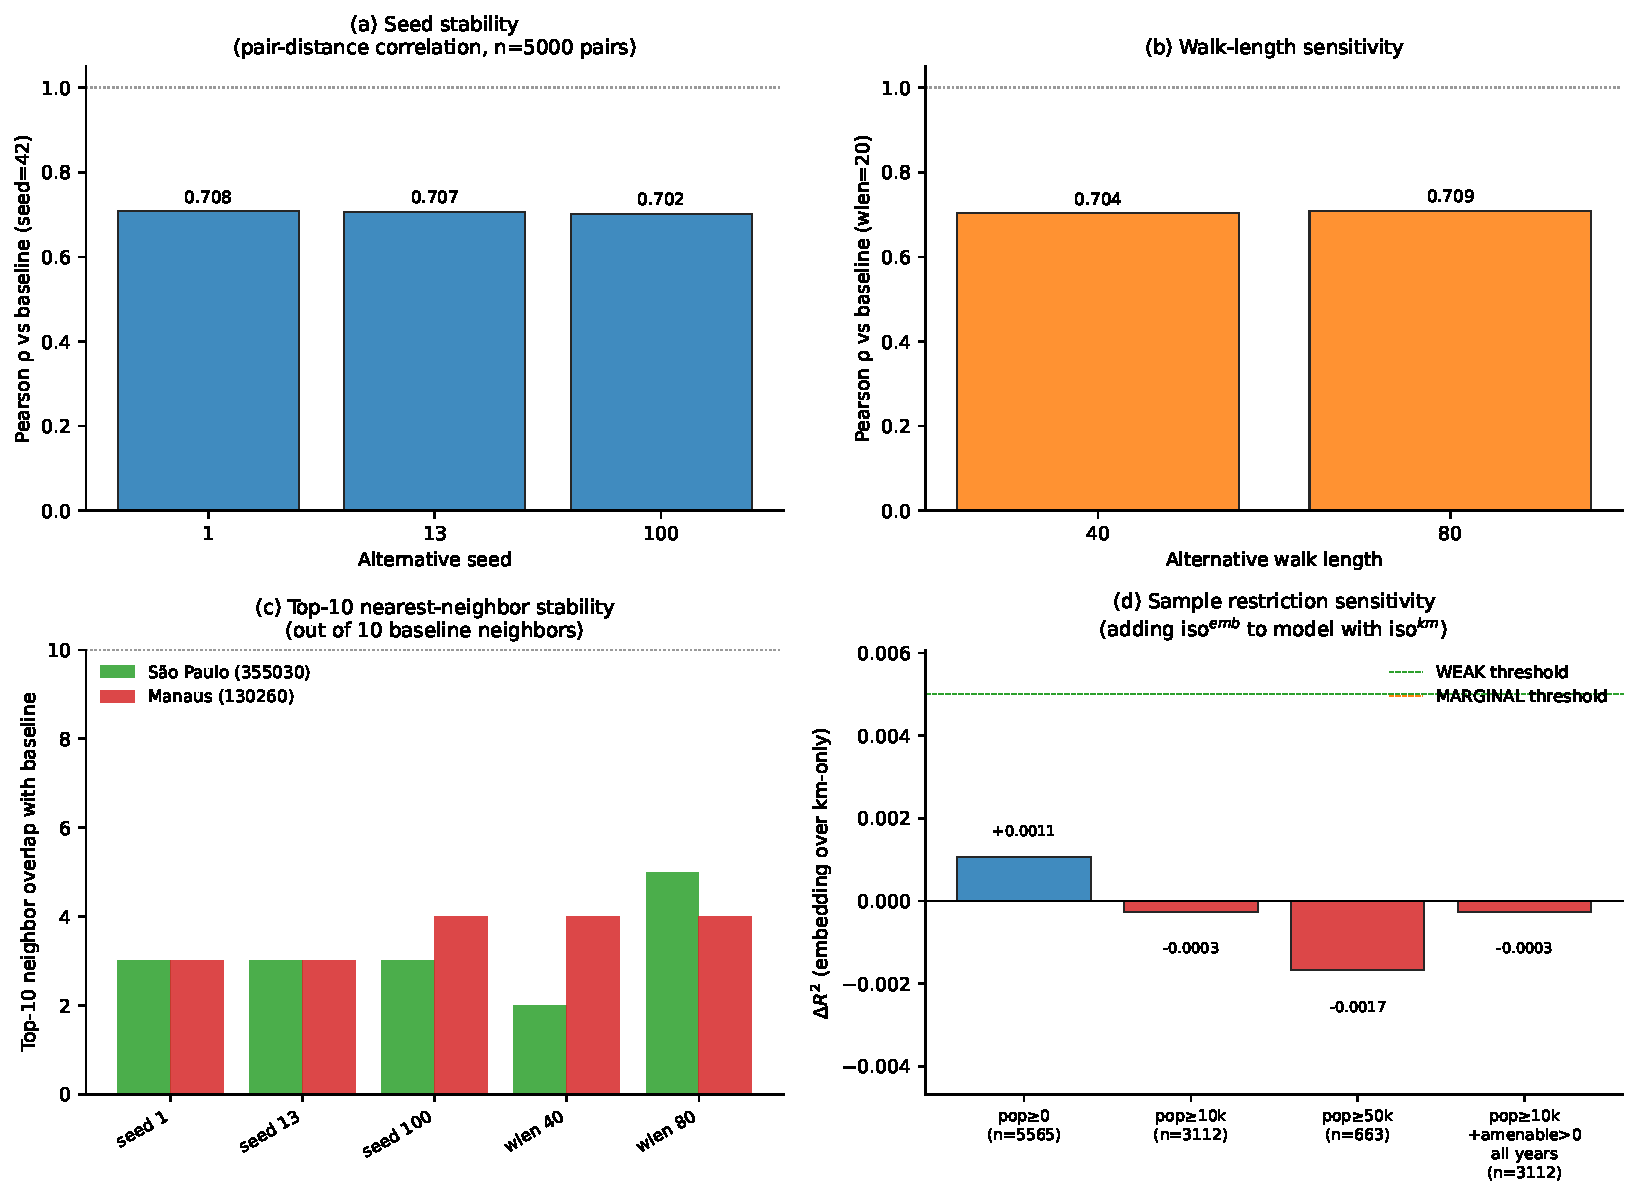
\includegraphics[width=0.95\textwidth]{../04_figures/fig_robustness.pdf}
    \caption{Robustness battery for the embedding and the predictive
    null. (a) Pearson correlation of pair-distance under three
    alternative seeds vs.\ baseline. (b) Same for two alternative walk
    lengths. (c) Top-10 nearest-neighbor overlap with baseline for
    São Paulo and Manaus. (d) $\Delta R^2$ from adding embedding
    isolation to the geographic-isolation model, by sample restriction.}
    \label{fig:robustness}
\end{figure}

\paragraph{Seed stability.}
We re-train the bipartite embedding under three additional seeds
($\{1, 13, 100\}$ in addition to the baseline $42$) holding
hyperparameters fixed, and compute the Pearson correlation between
embedding distance under the baseline and each alternative seed on
$5{,}000$ municipality pairs randomly selected with a fixed seed (so
that the same pairs are queried across all comparisons). The
correlations are $0.71$ (seed $1$), $0.71$ (seed $13$), and $0.70$
(seed $100$). The top-$10$ embedding-cosine neighbors of São Paulo
overlap with the baseline list in $3\text{--}5$ out of $10$
positions; for Manaus, $3\text{--}4$ out of $10$. Although individual
neighbor lists are not identical across seeds, the substantive
geographic signal is preserved: the metropolitan ABC and the Manaus
ribeirinho cluster always dominate the respective top-$10$, only the
relative ordering of municipalities within each cluster is unstable.
The $0.7$ pair-distance correlation indicates that the random seed
captures genuine specification uncertainty in the embedding; the
divergence map therefore should be read at the level of regional
patterns, not at the level of any individual municipality's exact rank.

\paragraph{Walk-length sensitivity.}
We re-train the embedding with walk length $\ell \in \{40, 80\}$ in
addition to the baseline $\ell = 20$, holding seed and other
hyperparameters fixed. Pair-distance correlations against baseline
are $0.70$ ($\ell = 40$) and $0.71$ ($\ell = 80$). The $\ell = 80$
specification yields slightly higher top-$10$ overlap with baseline
($5/10$ for São Paulo, $4/10$ for Manaus) than $\ell = 40$
($2/10$, $4/10$). The correlation pattern suggests that the dominant
source of embedding variation is the random walk realization, not the
walk length, once $\ell \geq 20$.

\paragraph{Alternative high-complexity definitions.}
The baseline defines a high-complexity hospital as any hospital with
an active SUS habilitation in any of seven categories. We test two
alternatives:

\textit{(i) Narrow definition: oncology and cardiology only.}
Restricting the high-complexity set to hospitals holding habilitations
in \textsc{onco} or \textsc{cardio} ($n = 4{,}725$ hospitals), the
Spearman rank-correlation of the resulting $\isoemb$ measure against
the baseline is $0.33$. This is a substantial decrease, indicating
that the choice of high-complexity definition matters for the
isolation metric. The narrow definition shrinks the eligible
hospital set by roughly $50\%$ and many municipalities switch nearest
hospitals as a consequence.

\textit{(ii) Long-lived habilitations: $\geq 24$ months active.}
Restricting to hospitals whose habilitation was active in at least
$24$ months during the panel window screens out short-lived
administrative classifications. The resulting $\isoemb$ has Spearman
$0.92$ with baseline. The choice of activity-duration threshold is
relatively innocuous.

The implication is that the network-revealed isolation measure is
robust to the activity-duration cut but sensitive to the categorical
breadth of the high-complexity definition. A reader interpreting the
divergence map should bear in mind that the metric reflects access to
the specific subset of services covered by the included habilitations;
applications targeting specific clinical conditions should re-derive
the metric over the relevant restricted hospital set.

\paragraph{Sample restriction sensitivity.}
The mortality regression in Section \ref{sec:results-mortality} uses
the sample of municipalities with mean population $\geq 10{,}000$,
yielding $n = 3{,}112$ observations. We re-run the regression on three
additional samples:
\begin{itemize}
    \item $n = 5{,}565$ (the unrestricted sample): $\Delta R^2$ from
        adding embedding-isolation to the geographic-isolation model
        is $+0.001$.
    \item $n = 663$ (mean population $\geq 50{,}000$): $\Delta R^2 =
        -0.002$.
    \item $n = 3{,}112$ (mean population $\geq 10{,}000$ \emph{and}
        non-zero amenable death count in every year of the panel):
        $\Delta R^2 = -0.0003$ (statistically indistinguishable from
        the baseline restriction).
\end{itemize}
The qualitative null is robust across these samples. Notably, the
sign of the $\Delta R^2$ flips slightly positive when small
municipalities are included; we interpret this as an artifact of the
SIM under-reporting gradient discussed in Section
\ref{sec:discussion}: the embedding captures sub-population structure
that, combined with the mechanical relationship between observed
amenable mortality and SIM-coverage gradients, produces a small
predictive gain in the smallest municipalities. This pattern strengthens
rather than weakens the methodological warning: the cross-sectional
regression is informative about observed amenable mortality, not about
the underlying mortality the access measure should predict.
